\section{INTEGRATION STRATEGY}
\subsection{Entry Criteria} 
Before the integration testing can begin, both the RASD and the DD must be completed. Furthermore at least the 80\% of the lines of the code of all components must have been tested with a Unit Test. We strongly suggest the Junit testing framework for Unit Testing.
\subsection{Elements to be Integrated} 
As we have described in the DD, the main components of the system are:
\begin{itemize}
\item Web Client GUI
\item Mobile Client GUI
\item Driver Client GUI
\item Service Manager 
\item HTTP Server
\item Request Handler
\item DBMS
\end{itemize}

In turn, the Service Manager is composed of:
\begin{itemize}
\item Car Manager
\item User Manager
\item Position Manager
\item Fee Manager
\end{itemize}
\noindent
For a further description of the components refer to the Design Document. 
\newline 
Of course, because before the Service Manager can be integrated with other components, the components that compose it have to be integrated.


\subsection{Integration Testing Strategy} 

We have chosen for the Integration Testing a \textbf{bottom up} approach. This means that the integration will regard first the low-level components. For this type of testing, because we start from the low level components, we will need some \textbf{drivers}. These are temporary modules that simulate the behaviour of the higher level components and do the calls of the functions of lower level components. \newline
That reason why we have chosen the bottom-up approach are:

\begin{itemize}
\item The lowest level component of our system is the DBMS, impletemented with MySQL 5.6. MySQL is a well-known software component that is available on the market. So the DBMS is ready to use and is a robust starting point for the Integration Testing. Starting from this we can begin to integrate the components of the Backend of our system, that essentialy is the Service Manager component. 
\item The low level components that compose the Backend of our service are the biggest part of our system and all the other components depends on them. Because of this importance of the low level components, the best choice is to start from them and, when it's sure that they work well together, integrate the other components.
\end{itemize}  

When the integration testing regards the Service Manager, the bottom up approach will be mixed with the \textbf{functional testing} approach. With functional testing, not the entire components are tested, but only some functionalities of them. In our case, when the components that compose the Service Manager will be tested together with the Service, only some functionalities of the Service Manager will be tested, that are the ones that call the specific subcomponent that is being tested.
\subsection{Sequence of Component/Function Integration} 
\subsubsection{Software Integration Sequence}
Because we have chosen a bottom up approach, the first components to be tested are the low level ones, so the ones that compose the Service Manager. After we have completed the integration for the subcomponents of the Service Manager, we will integrate the components that are directly interfaced with that subsystem, that are the Car Manager and the Request Manager. At the end, we will integrate the remaining front-end components, that are the Web Client and the Mobile Client.
At each step of the integration, a driver for the new component to be integrated has to be constructed. When the integration testing regarding that component stops, the driver is replaced with the actual component.
\paragraph{Integration of the components of the Service Manager}
The strategy that we have chosen to follow for the integration testing between the subcomponents of the Service Manager and the Service Manager itself is a functional one. So it won't constructed a driver for all the functionalities of the Service Manager, but at every step a driver for the single functionality regarding the subcomponent that is being tested is constructed.
\subparagraph{Request Manager and User Manager}
The first components to be tested with the Service Manager are the ones that have a relation with the DBMS: the User Manager and the Reservation Manager. The first one has to manipulate data regarding the users and their accounts and the second one has to manipulate data regarding the cars. As we mentioned in the previous section, the DBMS is a component ready to use, so the User Manager and the Reservation Manager will be directly tested with the DBMS, without the construction of drivers. The tests with the DBMS have to precede those with the Service Manager \newline
The order in which the Reservation Manager and the User Manager are chosen doesn't matter. 

\begin{figure}[H]	
	\centering
	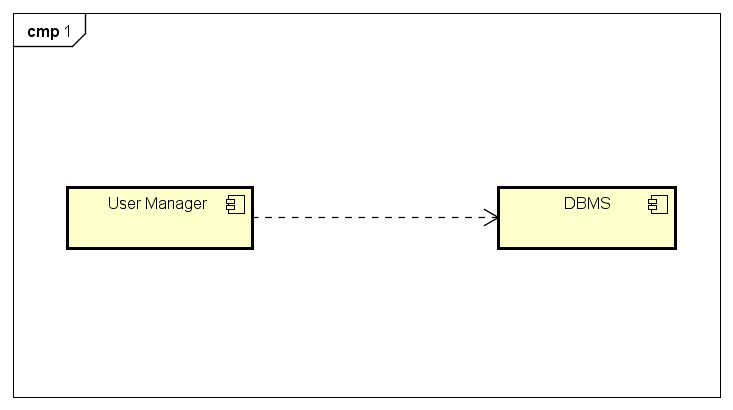
\includegraphics[width=\textwidth]{img/UserMan_DBMS_int}
	\caption{Integration of User Manager and DBMS}
\end{figure}

\begin{figure}[H]	
	\centering
	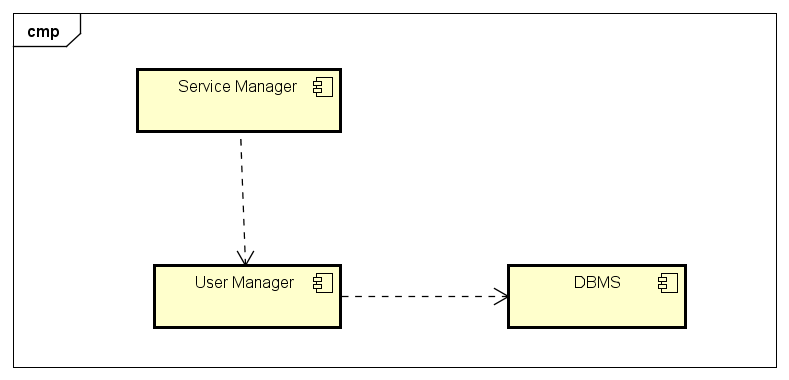
\includegraphics[width=\textwidth]{img/UserMan_SrvMan_int}
	\caption{Integration of User Manager and DBMS with Service Manager}
\end{figure}

\begin{figure}[H]	
	\centering
	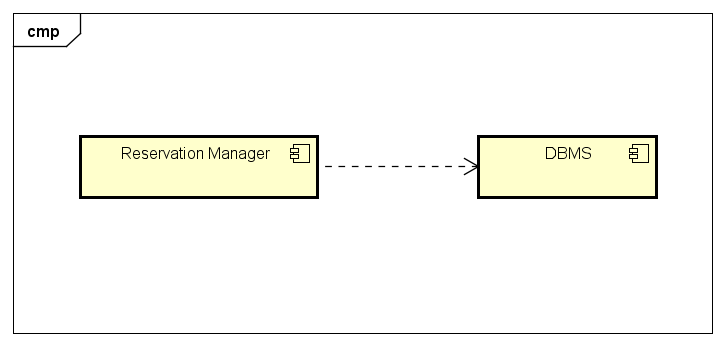
\includegraphics[width=\textwidth]{img/ResMan_DBMS_int}
	\caption{Integration of Reservation Manager and DBMS}
\end{figure}

\begin{figure}[H]	
	\centering
	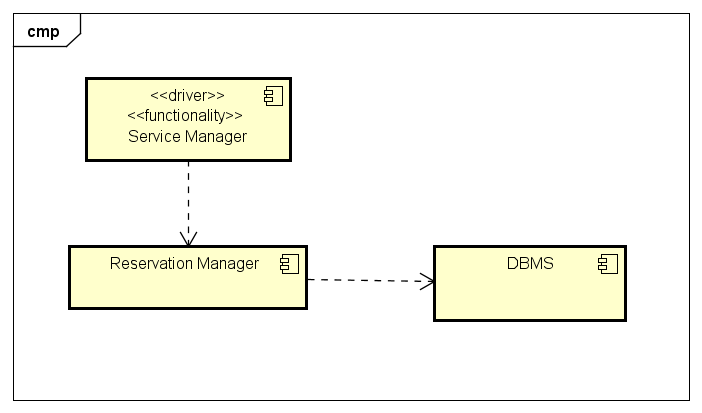
\includegraphics[width=\textwidth]{img/ResMan_SrvMan_int}
	\caption{Integration of Reservation Manager and DBMS with Service Manager}
\end{figure}
\subparagraph{Fee Manager}
The Fee Manager has to interact with payment systems, because it has the task of calculating the fee and charging the user. Because it would be hard and expensive using a real payment system, a stub simulating its functionalities is used. The tests with the Payment System stub have to precede the tests with the Service Manager. 


\begin{figure}[H]	
	\centering
	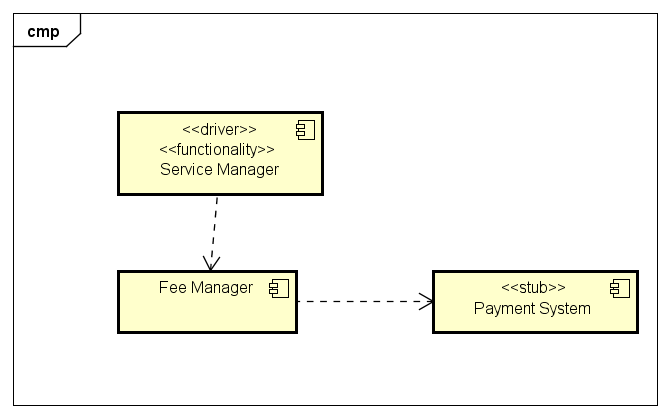
\includegraphics[width=\textwidth]{img/FeeMan_PaySys_int}
	\caption{Integration of Fee Manager and Payment System}
\end{figure}

\begin{figure}[H]	
	\centering
	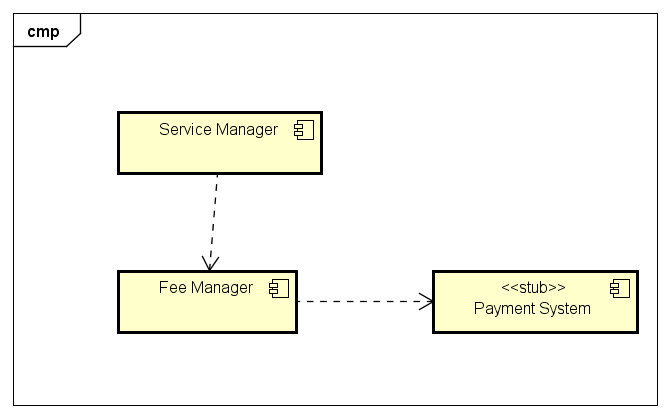
\includegraphics[width=\textwidth]{img/FeeMan_SrvMan_int}
	\caption{Integration of Fee Manager and Payment System with Service Manager}
\end{figure}

\subparagraph{Position Manager}
In addition to the Service Manager, the Position Manager has to interact also with the GPS software. Like the DBMS, the GPS software is a component found on the market and ready to use and so it can be tested directly with the Position Manager, without the construction of a driver. The tests with the GPS component have to precede the tests with the Service Manager.


\begin{figure}[H]	
	\centering
	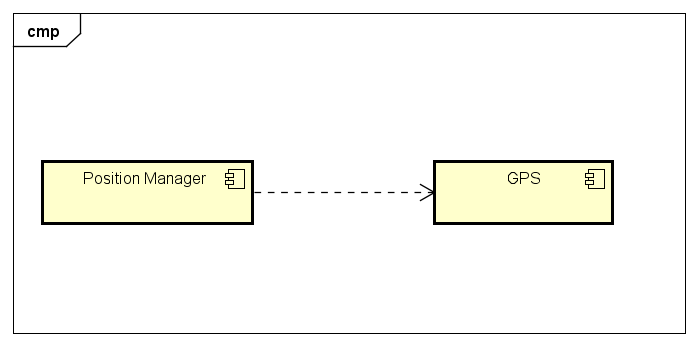
\includegraphics[width=\textwidth]{img/PosMan_GPS_int}
	\caption{Integration of Position Managere and GPS}
\end{figure}


\begin{figure}[H]	
	\centering
	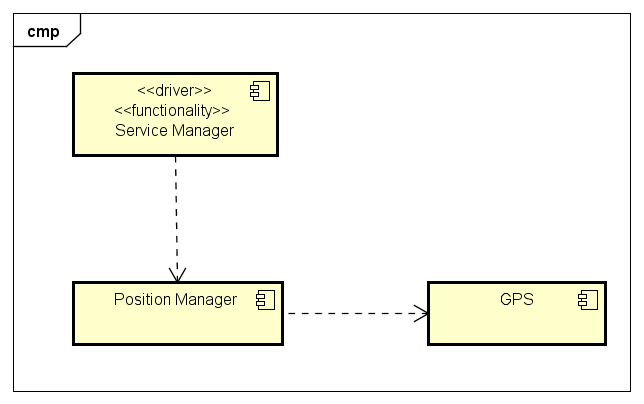
\includegraphics[width=\textwidth]{img/PosMan_SrvMan_int}
	\caption{Integration of Position Manager and GPS with Service Manager}
\end{figure}

\subparagraph{Car Manager}
The Car Manager is interfaced only with the Service Manager, so it is tested only with the driver of that component:

\begin{figure}[H]	
	\centering
	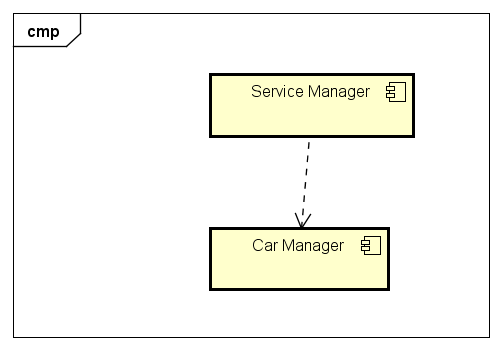
\includegraphics[width=\textwidth]{img/CarMan_SrvMan_int}
	\caption{Integration of Car Manager and Service Manager}
\end{figure}

\paragraph{Components interacting with the Service Manager}
After the integration tests on the subcomponents of the System Manager are completed, the Service Manager is ready to be integrated with higher level components. The testing of the subcomponents of the Service Manager ends here because those subcomponents implement functionalities that are independent with each other and so is sufficient to test them singularly together with the Service Manager and the external components they need.
\newline
So, after the completion of the test on the Service Manager, its driver is substituted by the actual component and this component will have to be tested with the Request Handler and the Car Manager, that are the components directly interfaced with the Service Manager.
First we choose to test the Service Manager with the Request Handler driver, because the Request Handler is the most critical component:


\begin{figure}[H]	
	\centering
	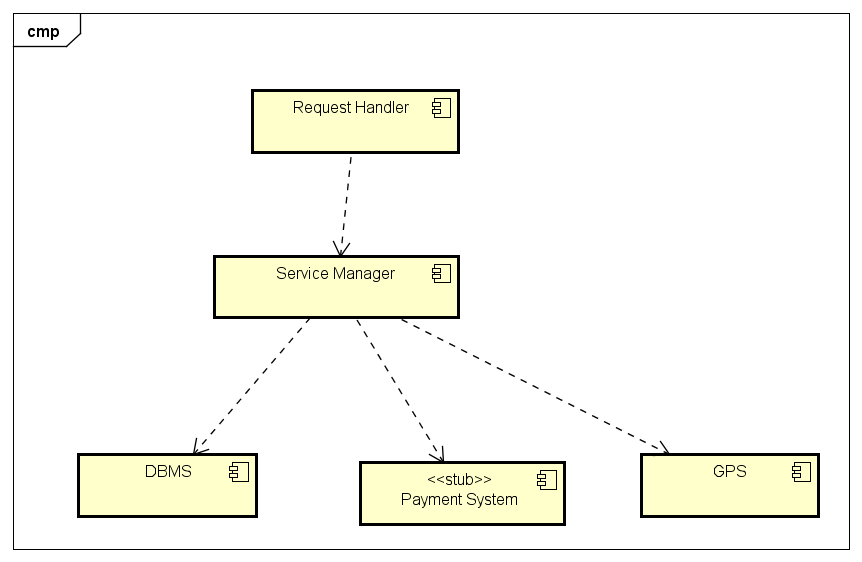
\includegraphics[width=\textwidth]{img/SrvMan_ReqHan_int}
	\caption{Integration of Request Handler with Service Manager, DBMS, GPS and Payment System}
\end{figure}

Then, the Service Manager is integrated with the OnBoard Device driver:


\begin{figure}[H]	
	\centering
	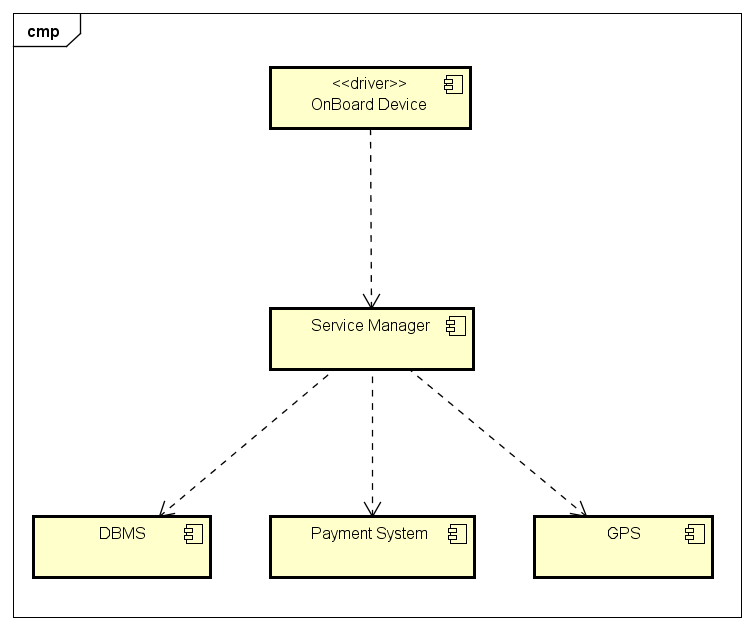
\includegraphics[width=\textwidth]{img/SrvMan_OnBoardDev_int}
	\caption{Integration of OnBoard Device with Service Manager, DBMS, GPS and Payment System}
\end{figure}

\paragraph{HTTP Server}
After the integration of the Request Handler and OnBoard Device, we can test the resulting subsystem with the HTTP Server driver. In particular the focus is on the interaction between the Request Handler and the HTTP Server:
\begin{figure}[H]	
	\centering
	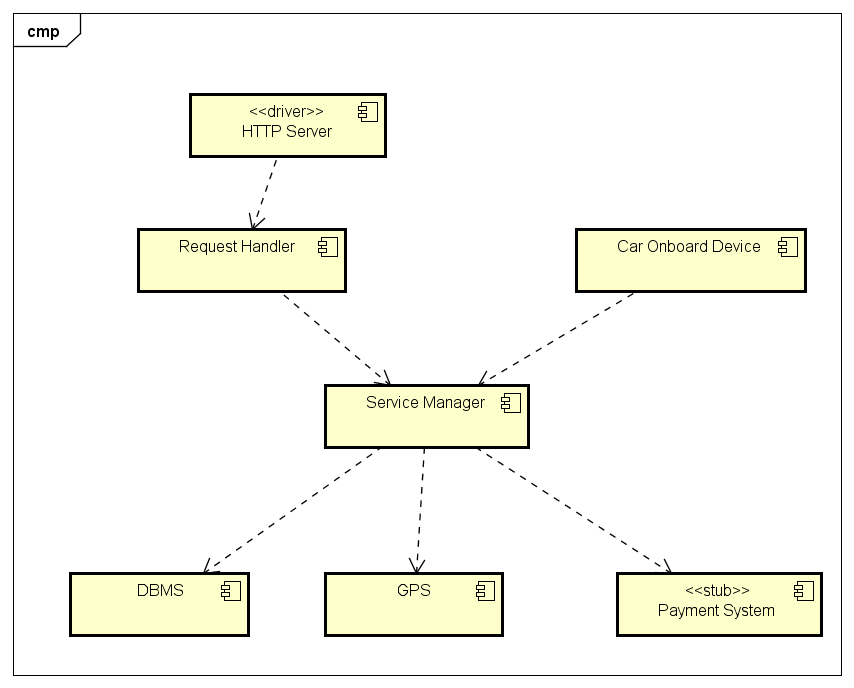
\includegraphics[width=\textwidth]{img/ReqHan_HTTP_int}
	\caption{Integration of HTTP Server and Subsystem including Request Handler, Service Manager, OnBoard Device, DBMS, GPS and Payment System}
\end{figure}

\paragraph{Frontend Components}
In the end, when the HTTP Server driver is substituted by the real component and this is tested with the drivers of the remaining two frontend components: the Mobile Client and the Web Client. The order in which this two components are chosen doesn't matter:
\begin{figure}[H]	
	\centering
	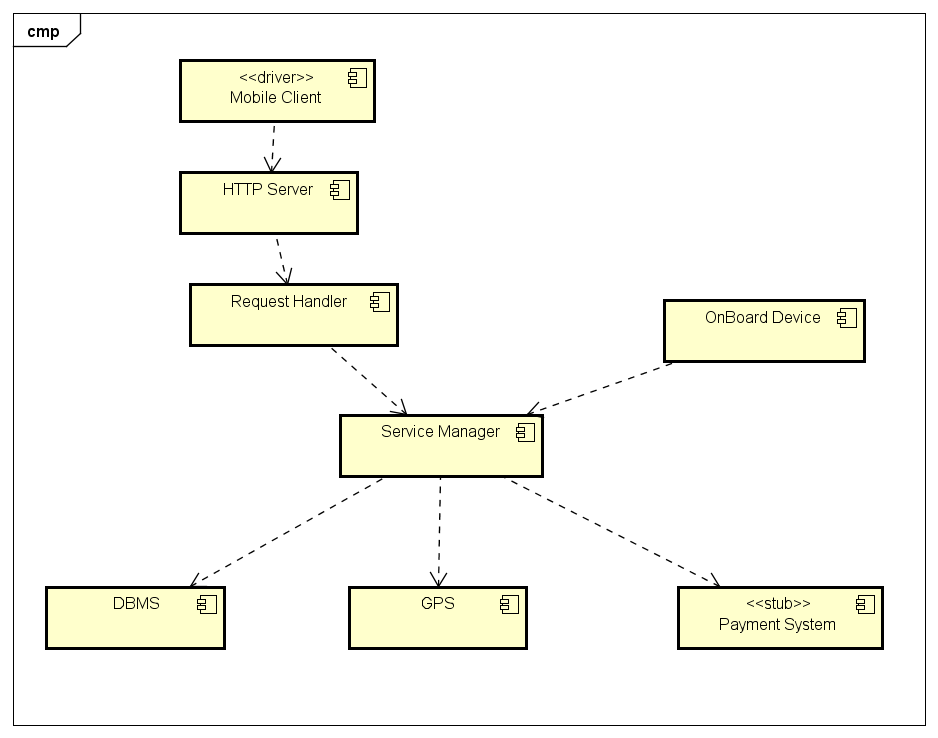
\includegraphics[width=\textwidth]{img/HTTP_MobCli_int}
	\caption{Integration of Mobile Client and Subsystem including HTTP Server, Request Handler, Service Manager, OnBoard Device, GPS, DBMS and Payment System}
\end{figure}

\begin{figure}[H]	
	\centering
	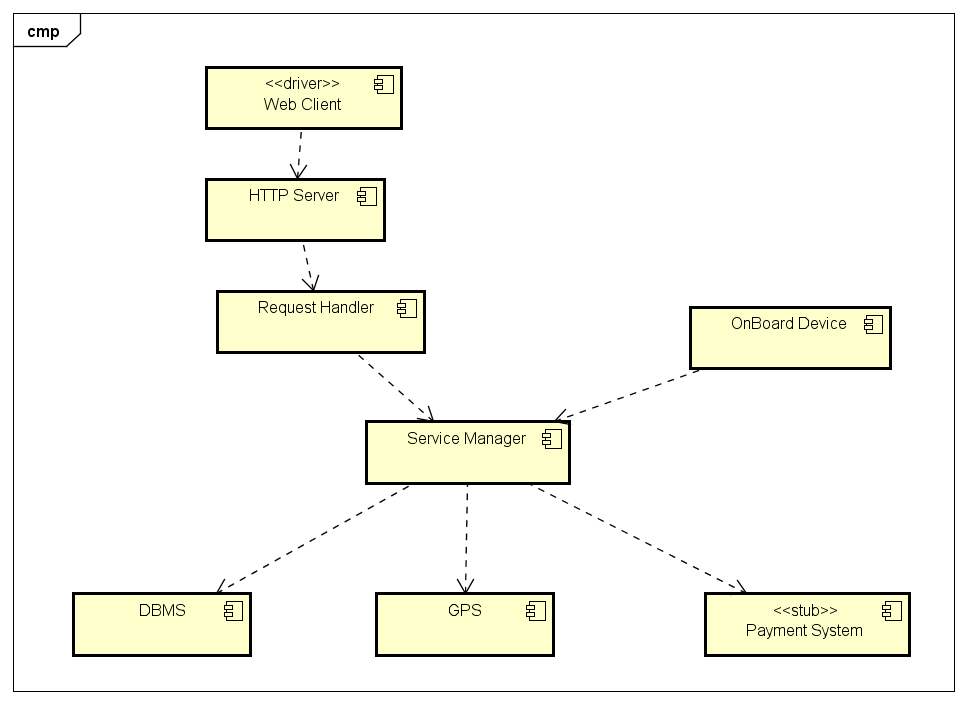
\includegraphics[width=\textwidth]{img/HTTP_WebCli_int}
	\caption{Integration of Web Client and Subsystem including HTTP Server, Request Handler, Service Manager, OnBoard Device, DBMS, GPS and Payment System}
\end{figure}

After these two integration tests, the all components of the system can be tested together.





